%------------------------
% Cover Letter Template
% Author : Shrikar Nakhye
% Position: Working Student AI Transformation (m/f/d)
% Company: BSH Hausgeräte GmbH
%------------------------

\documentclass[a4paper,10pt]{article}

\usepackage{latexsym}
\usepackage[empty]{fullpage}
\usepackage{titlesec}
\usepackage{marvosym}
\usepackage[usenames,dvipsnames]{color}
\usepackage{verbatim}
\usepackage{enumitem}
\usepackage[hidelinks]{hyperref}
\usepackage{fancyhdr}
\usepackage{tabularx}
\usepackage{graphicx}

\newlength{\origtextwidth}

\pagestyle{fancy}
\fancyhf{} % clear all header and footer fields
\fancyfoot{}
\renewcommand{\headrulewidth}{0pt}
\renewcommand{\footrulewidth}{0pt}

% Adjust margins & Fix footskip warning
\addtolength{\oddsidemargin}{-0.530in}
\addtolength{\evensidemargin}{-0.375in}
\addtolength{\textwidth}{1in}
\addtolength{\topmargin}{-.45in}
\addtolength{\textheight}{1in}
\setlength{\footskip}{3.60004pt}

\urlstyle{rm}

\raggedbottom
\raggedright
\setlength{\tabcolsep}{0in}

\begin{document}

%----------HEADING-----------------
\setlength{\origtextwidth}{\textwidth}
\definecolor{headerbg}{RGB}{242, 244, 247}
\vspace*{-\dimexpr\topmargin+1in\relax}
\noindent
\makebox[\origtextwidth][c]{%
  \colorbox{headerbg}{%
    \begin{minipage}{\paperwidth}
      \vspace*{25pt}
      \hspace{\dimexpr\oddsidemargin+1in\relax}%
      \begin{minipage}[c]{0.72\origtextwidth}
          \raggedright
          {\Huge \textbf{Shrikar Nakhye}} \\[6pt]
          \small
          Address: Bonn, Germany \\
          Email: \href{mailto:nakhyeshrikar@icloud.com}{nakhyeshrikar@icloud.com} \\
          Date of Birth: 30 August 2000 \\[6pt]
          \raisebox{-2pt}{
\includegraphics[height=10pt]{images/LinkedIn.png}}\ \href{https://www.linkedin.com/in/shrikar-nakhye-053262188/}{LinkedIn} \quad
          \raisebox{-2pt}{
\includegraphics[height=10pt]{images/github.png}}\ \href{https://github.com/ItsShriks}{GitHub} \quad
          \raisebox{-2pt}{
\includegraphics[height=10pt]{images/Google_Scholar.png}}\ \href{https://scholar.google.com/citations?user=-kVcoO8AAAAJ&hl=en}{Google Scholar}
      \end{minipage}%
      \hfill
      \begin{minipage}[c]{0.20\origtextwidth}
          \raggedleft
          {\setlength{\fboxsep}{0pt}\fbox{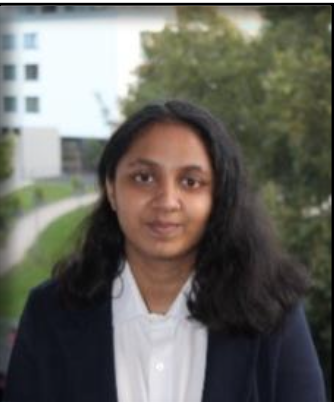
\includegraphics[width=2.5cm,height=3.3cm,keepaspectratio]{images/Self_Pic.jpg}}}
      \end{minipage}%
      \hspace{\dimexpr\oddsidemargin+1in\relax}%
      \vspace{15pt}
    \end{minipage}%
  }%
}

\vspace{25pt}
\hspace{0.015\textwidth}
\begin{minipage}{0.97\textwidth}

\hfill \today

\vspace{15pt}

\textbf{An:} \\
BSH Hausgeräte GmbH \\
Recruiting Team \\
Munich, Germany

\vspace{20pt}

\textbf{Betreff: Bewerbung als Working Student AI Transformation (m/w/d) -- Job-ID: 76044446}

\vspace{20pt}

Dear Hiring Team,

\vspace{10pt}

I am writing to express my keen interest in the Working Student AI Transformation position at BSH Hausgeräte GmbH (Job-ID: 76044446), available from August 2026. As a Master's student in Autonomous Systems at Hochschule Bonn-Rhein-Sieg with hands-on experience in AI, data analysis, and cross-functional project work, I am excited by the opportunity to contribute to BSH's digital transformation journey -- a company whose vision of intelligent home appliances I find genuinely inspiring.

\vspace{10pt}

What draws me to this role is the direct intersection of AI research, data harmonization, and enterprise system adoption -- areas where I have actively developed my skills:

\begin{itemize}[leftmargin=*]
    \item \textbf{AI Research \& Evaluation}: As a Research Assistant at HBRS and core member of the b-it bots @Home robotics team, I continuously research, evaluate, and benchmark AI and machine learning solutions -- ranging from deep learning perception models (PyTorch) to large language model APIs (DeepSeek, SAM3). I am comfortable documenting findings and communicating them clearly to interdisciplinary teams.
    \item \textbf{Data Analysis \& Visualization}: I work extensively with Python's data stack (NumPy, Pandas, Plotly) to process, analyze, and visualize complex datasets. In my work at Hochschule Bonn-Rhein-Sieg, I maintained structured experiment logs and evaluation reports, and developed scripts to inspect and validate sensor data consistency -- directly transferable to the reporting and data harmonization tasks in this role.
    \item \textbf{Data Cleansing \& Master Data Quality}: At Navilan Solutions, I developed an application to process and validate enterprise business documents -- identifying structural inconsistencies in JSON/YAML-structured data and enforcing data quality standards. This analytical approach to identifying and correcting data inconsistencies aligns closely with the customer master data harmonization work described for this position.
    \item \textbf{Documentation \& Communication}: I have authored technical documentation and research communications across my academic and professional roles, including four peer-reviewed publications. I understand the importance of clear, structured communication to support system adoption and stakeholder alignment -- exactly what is needed for the S/4HANA roll-in and change management tasks.
    \item \textbf{Cross-functional Collaboration}: As a Scrum Master at Sakar Robotics, I coordinated a 10-engineer team across technical and non-technical stakeholders. I am experienced in bridging departments and ensuring that digital transformation projects progress with clear interlinkages and shared understanding.
\end{itemize}

\vspace{10pt}

I am fluent in both English (C2) and German (B2), and I am actively expanding my German language proficiency -- enabling me to contribute effectively in BSH's bilingual working environment. I am available to start from August 2026 and am fully open to the hybrid working model described.

\vspace{10pt}

The opportunity to work within BSH's AI Transformation team -- applying my technical background to real-world enterprise challenges while growing in a structured, internationally renowned organization -- is a highly motivating prospect. I am eager to bring my analytical mindset, hands-on AI experience, and clear communication skills to your team.

\vspace{10pt}

Thank you sincerely for your time and consideration. I would be delighted to discuss how my profile aligns with your team's needs.

\vspace{25pt}

Sincerely,

\vspace{20pt}
Shrikar Nakhye

\end{minipage}

\end{document}
